\documentclass{article}\usepackage[]{graphicx}\usepackage[]{color}
%% maxwidth is the original width if it is less than linewidth
%% otherwise use linewidth (to make sure the graphics do not exceed the margin)
\makeatletter
\def\maxwidth{ %
  \ifdim\Gin@nat@width>\linewidth
    \linewidth
  \else
    \Gin@nat@width
  \fi
}
\makeatother

\definecolor{fgcolor}{rgb}{0.345, 0.345, 0.345}
\newcommand{\hlnum}[1]{\textcolor[rgb]{0.686,0.059,0.569}{#1}}%
\newcommand{\hlstr}[1]{\textcolor[rgb]{0.192,0.494,0.8}{#1}}%
\newcommand{\hlcom}[1]{\textcolor[rgb]{0.678,0.584,0.686}{\textit{#1}}}%
\newcommand{\hlopt}[1]{\textcolor[rgb]{0,0,0}{#1}}%
\newcommand{\hlstd}[1]{\textcolor[rgb]{0.345,0.345,0.345}{#1}}%
\newcommand{\hlkwa}[1]{\textcolor[rgb]{0.161,0.373,0.58}{\textbf{#1}}}%
\newcommand{\hlkwb}[1]{\textcolor[rgb]{0.69,0.353,0.396}{#1}}%
\newcommand{\hlkwc}[1]{\textcolor[rgb]{0.333,0.667,0.333}{#1}}%
\newcommand{\hlkwd}[1]{\textcolor[rgb]{0.737,0.353,0.396}{\textbf{#1}}}%

\usepackage{framed}
\makeatletter
\newenvironment{kframe}{%
 \def\at@end@of@kframe{}%
 \ifinner\ifhmode%
  \def\at@end@of@kframe{\end{minipage}}%
  \begin{minipage}{\columnwidth}%
 \fi\fi%
 \def\FrameCommand##1{\hskip\@totalleftmargin \hskip-\fboxsep
 \colorbox{shadecolor}{##1}\hskip-\fboxsep
     % There is no \\@totalrightmargin, so:
     \hskip-\linewidth \hskip-\@totalleftmargin \hskip\columnwidth}%
 \MakeFramed {\advance\hsize-\width
   \@totalleftmargin\z@ \linewidth\hsize
   \@setminipage}}%
 {\par\unskip\endMakeFramed%
 \at@end@of@kframe}
\makeatother

\definecolor{shadecolor}{rgb}{.97, .97, .97}
\definecolor{messagecolor}{rgb}{0, 0, 0}
\definecolor{warningcolor}{rgb}{1, 0, 1}
\definecolor{errorcolor}{rgb}{1, 0, 0}
\newenvironment{knitrout}{}{} % an empty environment to be redefined in TeX

\usepackage{alltt}

\title{Problem Set 2}
\author{Tony Lashley}
\date{April 13, 2015}

\usepackage{natbib}
\usepackage{graphicx}
\graphicspath{{/Users/Tony/Pictures/}}
\IfFileExists{upquote.sty}{\usepackage{upquote}}{}
\begin{document}
\maketitle

\section{Machinery for the Schelling Model}
\subsection{Write a function that calculates distances between coordinate points}
\begin{knitrout}
\definecolor{shadecolor}{rgb}{0.969, 0.969, 0.969}\color{fgcolor}\begin{kframe}
\begin{alltt}
\hlstd{individual} \hlkwb{<-} \hlkwd{c}\hlstd{(}\hlkwc{x} \hlstd{=} \hlnum{0}\hlstd{,}\hlkwc{y} \hlstd{=} \hlnum{0}\hlstd{)}
\hlkwd{print}\hlstd{(individual)}
\end{alltt}
\begin{verbatim}
## x y 
## 0 0
\end{verbatim}
\begin{alltt}
\hlstd{neighbors} \hlkwb{=} \hlkwd{matrix}\hlstd{(}\hlnum{1}\hlopt{:}\hlnum{8}\hlstd{,} \hlkwc{ncol} \hlstd{=} \hlnum{2}\hlstd{,} \hlkwc{byrow} \hlstd{= T)}
\hlkwd{print}\hlstd{(neighbors)}
\end{alltt}
\begin{verbatim}
##      [,1] [,2]
## [1,]    1    2
## [2,]    3    4
## [3,]    5    6
## [4,]    7    8
\end{verbatim}
\begin{alltt}
\hlkwd{colnames}\hlstd{(neighbors)} \hlkwb{<-} \hlkwd{c}\hlstd{(}\hlstr{"X"}\hlstd{,}\hlstr{"Y"}\hlstd{)}
\hlstd{dstances} \hlkwb{=} \hlkwd{matrix}\hlstd{(}\hlkwc{ncol} \hlstd{=} \hlnum{3}\hlstd{,} \hlkwc{byrow} \hlstd{= T)}
\hlkwd{colnames}\hlstd{(dstances)} \hlkwb{<-} \hlkwd{c}\hlstd{(}\hlstr{"X"}\hlstd{,}\hlstr{"Y"}\hlstd{,} \hlstr{"Pythgorean"}\hlstd{)}

\hlstd{f1} \hlkwb{<-} \hlkwa{function}\hlstd{(}\hlkwc{individual}\hlstd{,} \hlkwc{neighbors}\hlstd{)\{}

  \hlkwa{for} \hlstd{(i} \hlkwa{in} \hlnum{1}\hlopt{:}\hlkwd{nrow}\hlstd{(neighbors))\{}

    \hlstd{neighbor_longitude} \hlkwb{=} \hlstd{neighbors[i,}\hlnum{1}\hlstd{]}
    \hlcom{## Find your neighbor's longitude}
    \hlstd{neighbor_latitude} \hlkwb{=}  \hlstd{neighbors[i,}\hlnum{2}\hlstd{]}
    \hlcom{## Find your neighbor's latitude}
    \hlstd{individual_longitude} \hlkwb{=} \hlstd{individual[}\hlnum{1}\hlstd{]}
    \hlcom{## Find your own longitude}
    \hlstd{individual_latitude} \hlkwb{=}  \hlstd{individual[}\hlnum{2}\hlstd{]}
    \hlcom{## Find your own latitude}

    \hlstd{lftrghtdstance} \hlkwb{=} \hlkwd{abs}\hlstd{(neighbor_longitude} \hlopt{-} \hlstd{individual_longitude)}
    \hlcom{## Find east/west distance between indiv. and neighbor}
    \hlstd{updowndstance} \hlkwb{=} \hlkwd{abs}\hlstd{(neighbor_latitude} \hlopt{-} \hlstd{individual_latitude)}
    \hlcom{## Find north/south distance between indiv. and neighbor}
    \hlstd{pyth} \hlkwb{=} \hlkwd{sqrt}\hlstd{(((lftrghtdstance)}\hlopt{^}\hlnum{2}\hlstd{)} \hlopt{+} \hlstd{((updowndstance)}\hlopt{^}\hlnum{2}\hlstd{))}
    \hlcom{## Find Euclidian distance}
    \hlstd{currentdistance} \hlkwb{=} \hlkwd{c}\hlstd{(lftrghtdstance,updowndstance,pyth)}
    \hlcom{## Make vector with Manhattan and Euclidian distances}


    \hlstd{dstances} \hlkwb{<-} \hlkwd{rbind}\hlstd{(dstances, currentdistance)}
    \hlcom{## Add vector as row in matrix of distances}
  \hlstd{\}}

  \hlkwd{return}\hlstd{(dstances)}
\hlstd{\}}

\hlkwd{f1}\hlstd{(individual, neighbors)}
\end{alltt}
\begin{verbatim}
##                  X  Y Pythgorean
##                 NA NA         NA
## currentdistance  1  2   2.236068
## currentdistance  3  4   5.000000
## currentdistance  5  6   7.810250
## currentdistance  7  8  10.630146
\end{verbatim}
\end{kframe}
\end{knitrout}

\subsection{Write a function that simulates Schelling's Segregation model}
\begin{knitrout}
\definecolor{shadecolor}{rgb}{0.969, 0.969, 0.969}\color{fgcolor}\begin{kframe}
\begin{alltt}
\hlkwd{library}\hlstd{(RANN)}
\hlkwd{library}\hlstd{(ggplot2)}
\hlkwd{library}\hlstd{(reshape2)}

\hlstd{testRacialPreferenceTable} \hlkwb{<-} \hlkwd{matrix}\hlstd{(}\hlnum{1}\hlopt{:}\hlnum{15}\hlstd{,} \hlkwc{ncol} \hlstd{=} \hlnum{5}\hlstd{,} \hlkwc{nrow} \hlstd{=} \hlnum{3}\hlstd{)}
\hlstd{testRacialPreferenceTable[}\hlnum{1}\hlstd{,]} \hlkwb{<-} \hlkwd{c}\hlstd{(}\hlstr{"R"}\hlstd{,}\hlnum{1}\hlstd{,} \hlnum{50}\hlstd{,} \hlnum{5}\hlstd{,} \hlnum{2}\hlstd{)}
\hlstd{testRacialPreferenceTable[}\hlnum{2}\hlstd{,]} \hlkwb{<-} \hlkwd{c}\hlstd{(}\hlstr{"G"}\hlstd{,} \hlnum{0}\hlstd{,} \hlnum{25}\hlstd{,} \hlnum{5}\hlstd{,} \hlnum{2}\hlstd{)}
\hlstd{testRacialPreferenceTable[}\hlnum{3}\hlstd{,]} \hlkwb{<-} \hlkwd{c}\hlstd{(}\hlstr{"B"}\hlstd{,} \hlopt{-}\hlnum{1}\hlstd{,} \hlnum{25}\hlstd{,} \hlnum{5}\hlstd{,} \hlnum{2}\hlstd{)}
\hlkwd{colnames}\hlstd{(testRacialPreferenceTable)} \hlkwb{<-} \hlkwd{c}\hlstd{(}\hlstr{"Color"}\hlstd{,} \hlstr{"Value"}\hlstd{,} \hlstr{"Pop."}\hlstd{,} \hlstr{"Test Pool Size"}\hlstd{,} \hlstr{"Racial Threshold"}\hlstd{)}

\hlstd{nR} \hlkwb{<-} \hlkwd{as.numeric}\hlstd{(testRacialPreferenceTable[}\hlnum{1}\hlstd{,}\hlstr{"Pop."}\hlstd{])}
\hlstd{nG} \hlkwb{<-} \hlkwd{as.numeric}\hlstd{(testRacialPreferenceTable[}\hlnum{2}\hlstd{,}\hlstr{"Pop."}\hlstd{])}
\hlstd{nB} \hlkwb{<-} \hlkwd{as.numeric}\hlstd{(testRacialPreferenceTable[}\hlnum{3}\hlstd{,}\hlstr{"Pop."}\hlstd{])}

\hlstd{n} \hlkwb{<-} \hlkwd{sum}\hlstd{(nR} \hlopt{+} \hlstd{nG} \hlopt{+} \hlstd{nB)}
\hlcom{## Find total population from summing each racial population}

\hlstd{Schelling} \hlkwb{<-} \hlkwa{function}\hlstd{(}\hlkwc{racialPreferenceTable} \hlstd{= testRacialPreferenceTable)\{}
  \hlkwd{set.seed}\hlstd{(}\hlnum{20016}\hlstd{)}
  \hlstd{LocationTable} \hlkwb{<-} \hlkwd{matrix}\hlstd{(}\hlkwc{ncol} \hlstd{=} \hlnum{3}\hlstd{)}
  \hlcom{## Initalizing table for initial neighborhood coordinates}

  \hlkwa{for} \hlstd{(i} \hlkwa{in} \hlnum{1}\hlopt{:}\hlstd{nR)\{}
    \hlstd{x} \hlkwb{<-} \hlkwd{runif}\hlstd{(}\hlnum{1}\hlstd{,} \hlkwc{min}\hlstd{=}\hlnum{0}\hlstd{,} \hlkwc{max}\hlstd{=}\hlnum{1}\hlstd{)}
    \hlcom{## Generate random X coordinate between 0 and 1 for point}
    \hlstd{y} \hlkwb{<-} \hlkwd{runif}\hlstd{(}\hlnum{1}\hlstd{,} \hlkwc{min}\hlstd{=}\hlnum{0}\hlstd{,} \hlkwc{max}\hlstd{=}\hlnum{1}\hlstd{)}
    \hlcom{## Generate random Y coordinate between 0 and 1 for point}
    \hlstd{currentpointR} \hlkwb{=} \hlkwd{c}\hlstd{(}\hlnum{1}\hlstd{,x,y)}
    \hlcom{## Create vector with point coordinates, labeling point as red}
    \hlstd{LocationTable} \hlkwb{<-} \hlkwd{rbind}\hlstd{(LocationTable, currentpointR)}
    \hlcom{## Add red point to table of all neighborhood coordinates}
  \hlstd{\}}

  \hlkwa{for} \hlstd{(i} \hlkwa{in} \hlnum{1}\hlopt{:}\hlstd{nG)\{}
    \hlstd{x} \hlkwb{<-} \hlkwd{runif}\hlstd{(}\hlnum{1}\hlstd{,} \hlkwc{min}\hlstd{=}\hlnum{0}\hlstd{,} \hlkwc{max}\hlstd{=}\hlnum{1}\hlstd{)}
    \hlstd{y} \hlkwb{<-} \hlkwd{runif}\hlstd{(}\hlnum{1}\hlstd{,} \hlkwc{min}\hlstd{=}\hlnum{0}\hlstd{,} \hlkwc{max}\hlstd{=}\hlnum{1}\hlstd{)}

    \hlstd{currentpointG} \hlkwb{=} \hlkwd{c}\hlstd{(}\hlnum{0}\hlstd{,x,y)}

    \hlstd{LocationTable} \hlkwb{<-} \hlkwd{rbind}\hlstd{(LocationTable, currentpointG)}
  \hlstd{\}}

  \hlkwa{for} \hlstd{(i} \hlkwa{in} \hlnum{1}\hlopt{:}\hlstd{nB)\{}
    \hlstd{x} \hlkwb{<-} \hlkwd{runif}\hlstd{(}\hlnum{1}\hlstd{,} \hlkwc{min}\hlstd{=}\hlnum{0}\hlstd{,} \hlkwc{max}\hlstd{=}\hlnum{1}\hlstd{)}
    \hlstd{y} \hlkwb{<-} \hlkwd{runif}\hlstd{(}\hlnum{1}\hlstd{,} \hlkwc{min}\hlstd{=}\hlnum{0}\hlstd{,} \hlkwc{max}\hlstd{=}\hlnum{1}\hlstd{)}
    \hlstd{currentpointB} \hlkwb{=} \hlkwd{c}\hlstd{(}\hlopt{-}\hlnum{1}\hlstd{,x,y)}

    \hlstd{LocationTable} \hlkwb{<-} \hlkwd{rbind}\hlstd{(LocationTable, currentpointB)}
  \hlstd{\}}

  \hlstd{LocationTable} \hlkwb{<-} \hlstd{LocationTable[}\hlopt{-}\hlnum{1}\hlstd{,]}

  \hlstd{p} \hlkwb{<-} \hlkwd{qplot}\hlstd{(}\hlkwc{x} \hlstd{= LocationTable[,}\hlnum{2}\hlstd{],} \hlkwc{y} \hlstd{= LocationTable [,}\hlnum{3}\hlstd{],} \hlkwc{col} \hlstd{=} \hlkwd{ifelse}\hlstd{(LocationTable[,}\hlnum{1}\hlstd{]} \hlopt{< -}\hlnum{0.5}\hlstd{,} \hlstr{"green"}\hlstd{,} \hlkwd{ifelse}\hlstd{(LocationTable[,}\hlnum{1}\hlstd{]} \hlopt{<} \hlnum{0.5}\hlstd{,} \hlstr{"red"}\hlstd{,} \hlstr{"blue"}\hlstd{)))} \hlopt{+} \hlkwd{theme}\hlstd{(}\hlkwc{legend.position} \hlstd{=} \hlstr{"none"}\hlstd{)}

  \hlkwd{print}\hlstd{(p)}
\hlstd{\}}

\hlkwd{Schelling}\hlstd{(testRacialPreferenceTable)}
\end{alltt}
\end{kframe}
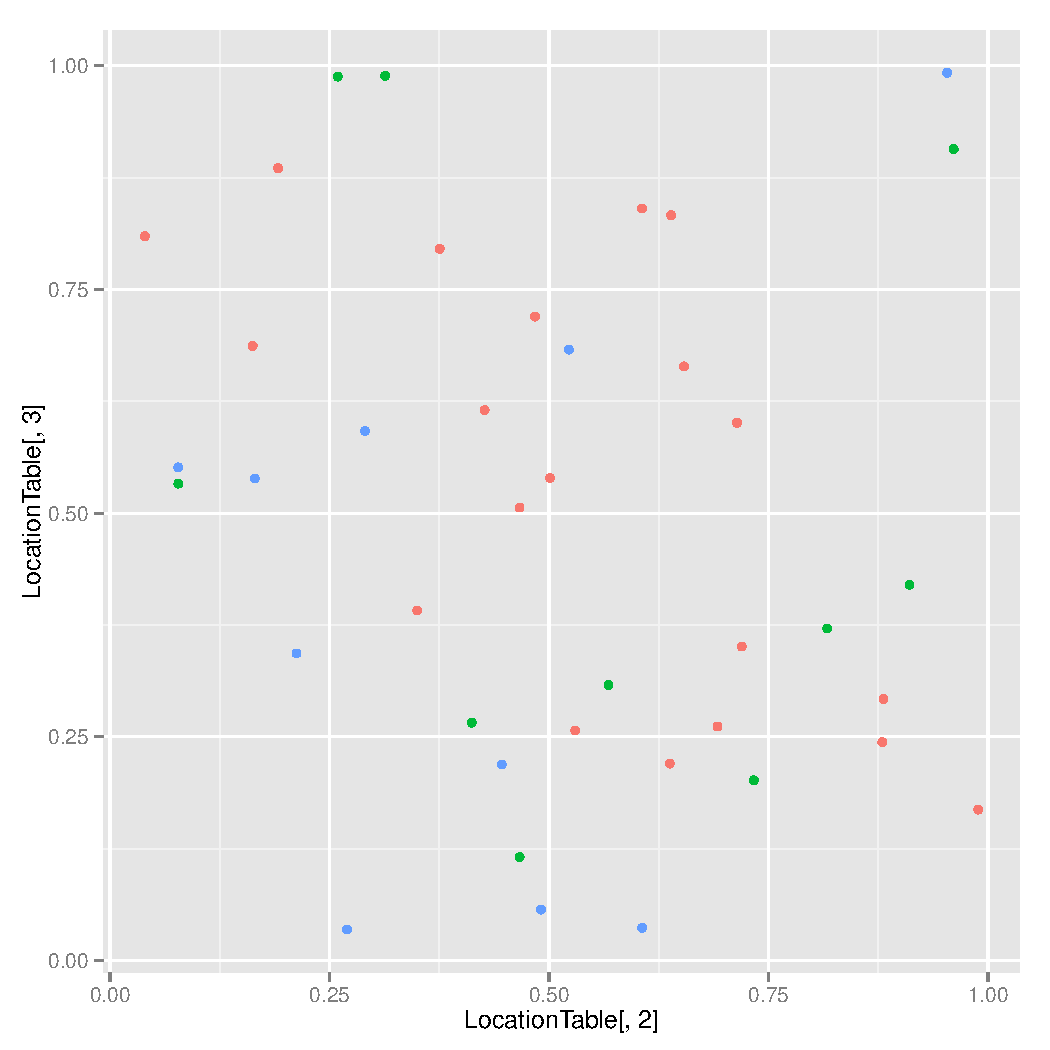
\includegraphics[width=\maxwidth]{figure/unnamed-chunk-2-1} 

\end{knitrout}



\end{document}
